
\documentclass[preprint,12pt]{elsarticle}

\usepackage[spanish]{babel}
\usepackage{amssymb}
\usepackage{graphicx}
\usepackage{lineno}
\usepackage[utf8]{inputenc}
\usepackage{url}
\usepackage{natbib}

\begin{document}
	
	\begin{frontmatter}

		\title{\huge  Laboratorio 01: Visualización de datos con
			Tableau }
		\author{	Tarqui Montalico,Risther(2017057469)}
		
		





\end{frontmatter}

%%INICIO Resumen
\section{Objetivo}
	
	Comprender la organización la información de nuestros datos de tal manera que todos los que los vean
	puedan comprender sus implicaciones y cómo actuar sobre ellos con claridad.
%%FIN Resumen


%%INICIO Introducción
\section{Introducción a Tableau}

	\begin{itemize}
	\item Instalación \\
	
		Dependiendo de la elección del producto, descargue el software en la computadora. Después de aceptar
		el acuerdo de licencia, puede verificar la instalación haciendo clic en el ícono de Tableau. Si aparece la
		siguiente pantalla, está listo para comenzar.
	 	\\	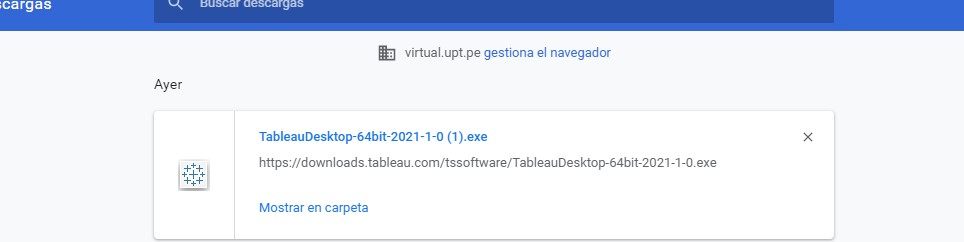
\includegraphics[width=10cm]{./IMAGENES/0.1}
	 	\\		\includegraphics[width=10cm]{./IMAGENES/0.2}
	\end{itemize}
%%FIN Introducción

\section{Comenzar}
	
	\subsection{Conexión a una fuente de datos}
		\begin{itemize}
			\item Importe los datos al espacio de trabajo de Tableau desde la computadora.

			
			\item En la pestaña Hojas, se verán tres hojas: Pedidos, Personas y Devoluciones. Sin embargo, nos
			centraremos solo en los datos de los pedidos. Haga doble clic en Hoja de pedidos y se abrirá
			como una hoja de cálculo. 
				
				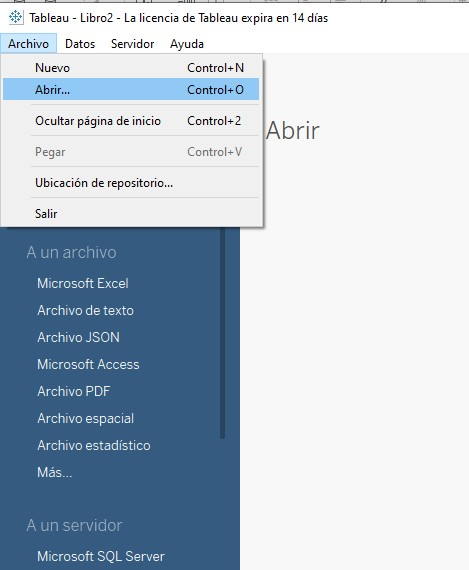
\includegraphics[width=10cm]{./IMAGENES/3.1}
			
			\item Observamos que las primeras tres filas de datos se ven un poco diferentes y no están en el
			formato deseado. Aquí utilizamos el intérprete de datos , también presente en la pestaña
			Hojas. Al hacer clic en él, obtenemos una hoja con un formato agradable. \\
				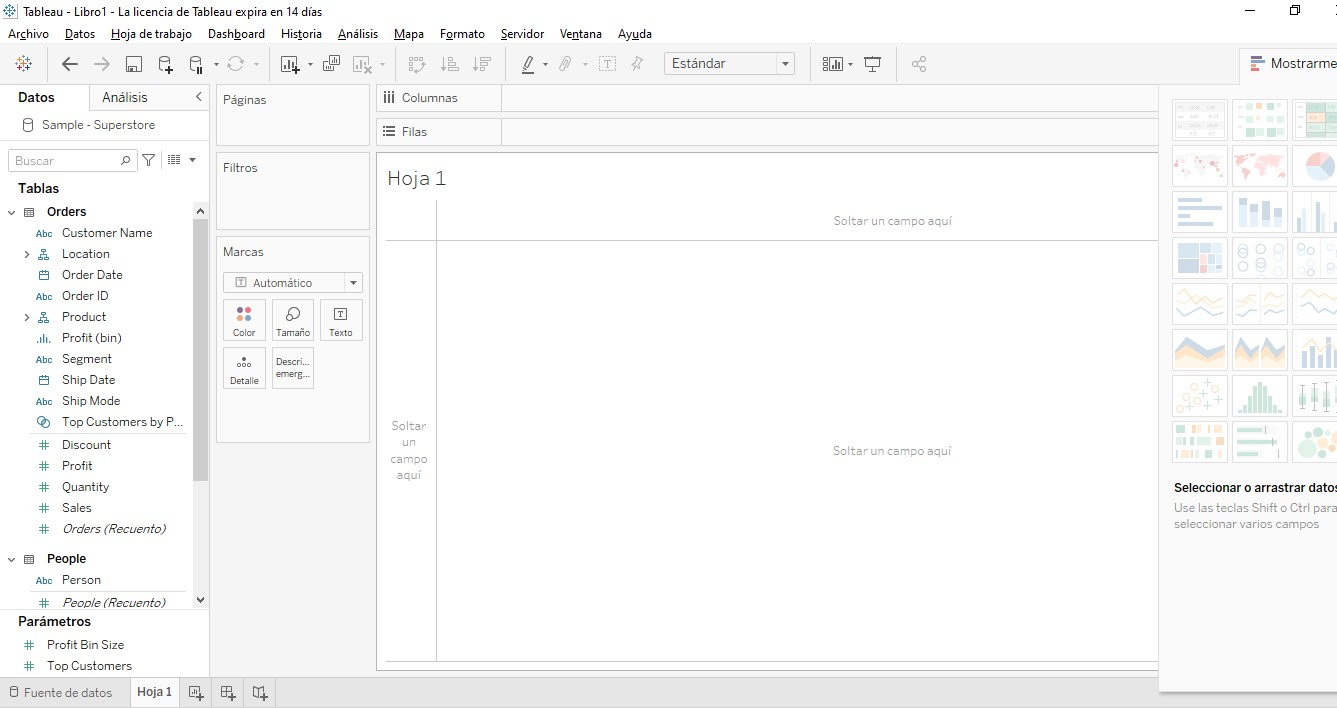
\includegraphics[width=10cm]{./IMAGENES/3.1.3}
		\end{itemize}
	
		\subsection{Crear una muestra}
		\begin{itemize}
			\item Vaya a la hoja de trabajo. Haga clic en la pestaña Sheet 1 en la parte inferior izquierda del
			espacio de trabajo del cuadro. 
			\\	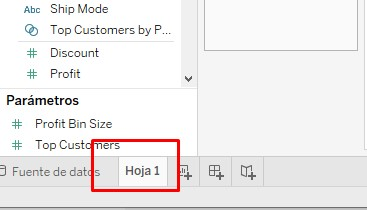
\includegraphics[width=10cm]{./IMAGENES/3.2.1}
			
			\item Una vez que esté en la hoja de trabajo, desde Dimensionsdebajo del panel Datos,
			arrastre Order Dateal estante Columna.
			\\	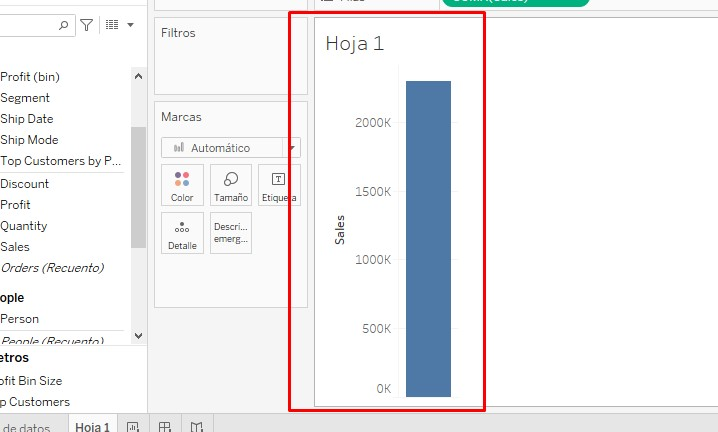
\includegraphics[width=10cm]{./IMAGENES/3.2.3}
			
			\item  Del mismo modo, desde la Measurespestaña, arrastre el Salescampo al estante Filas
			\\	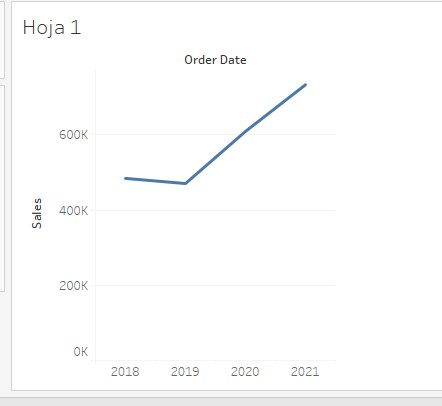
\includegraphics[width=10cm]{./IMAGENES/3.2.4}
		
		\end{itemize}
	
		\subsection{Refinando vista}
		\begin{itemize}
			\item Categoryestá presente en el panel Dimensiones. Arrástrelo al estante de columnas y colóquelo
			junto a YEAR(Order Date). El Categorydebe ser colocado a la derecha de Year. Al
			hacerlo, la vista cambia inmediatamente a un tipo de gráfico de barras desde una línea. El
			gráfico muestra el total Sales de cada Product año.
			Learn More
			\\	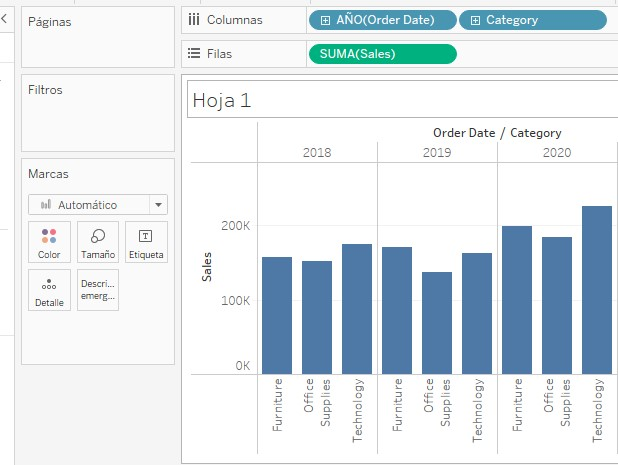
\includegraphics[width=10cm]{./IMAGENES/3.3.1}
			\item La vista por encima de Niza los espectáculos sales de category, por ejemplo, muebles, equipos
			de oficina, y la tecnología. También podemos inferir que las ventas de muebles están creciendo más
			rápido que las ventas de suministros de oficina, excepto en 2016. Por lo tanto, sería prudente centrar los
			esfuerzos de ventas en muebles en lugar de suministros de oficina. Pero los muebles son una categoría
			amplia y se componen de muchos elementos diferentes. ¿Cómo podemos identificar qué mueble está
			contribuyendo a las ventas máximas?
			\\	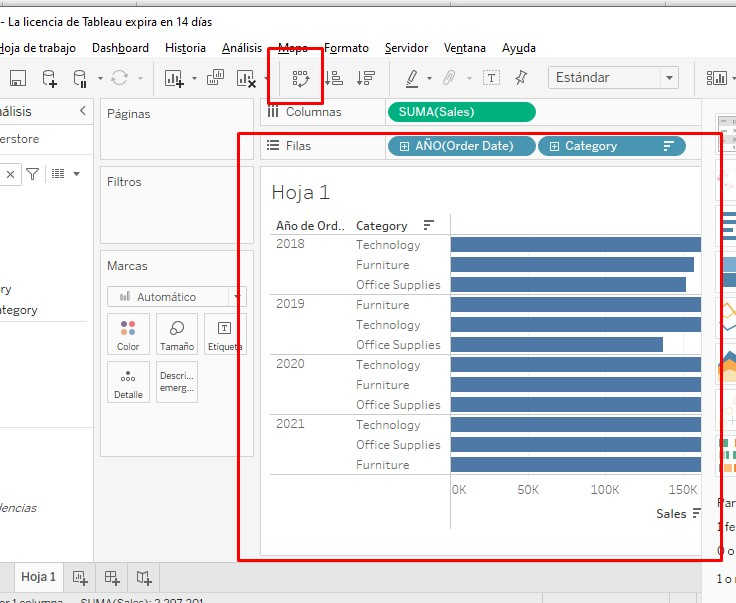
\includegraphics[width=10cm]{./IMAGENES/3.3.1.2}
		
			
			
		\end{itemize}
	\section
	


\section{Enfatizando los resultados}

	\subsection{Agregar filtros a la vista}
		\\	\includegraphics[width=10cm]{./IMAGENES/4.1}
	\subsection{Agregar colores a la vista}
		\\	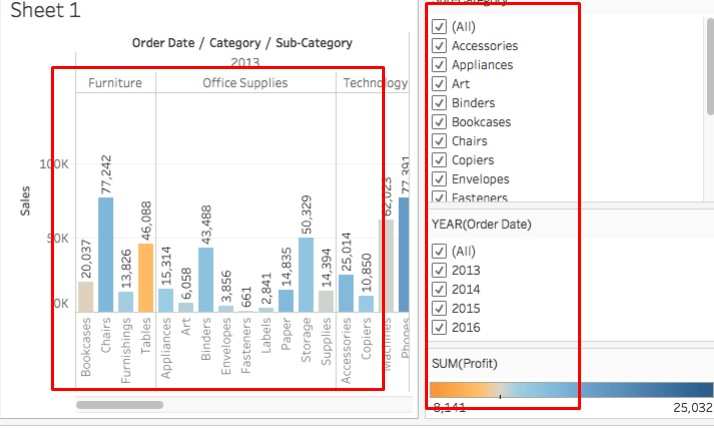
\includegraphics[width=10cm]{./IMAGENES/4.2}
	\subsection{Resultados clave}
		\\	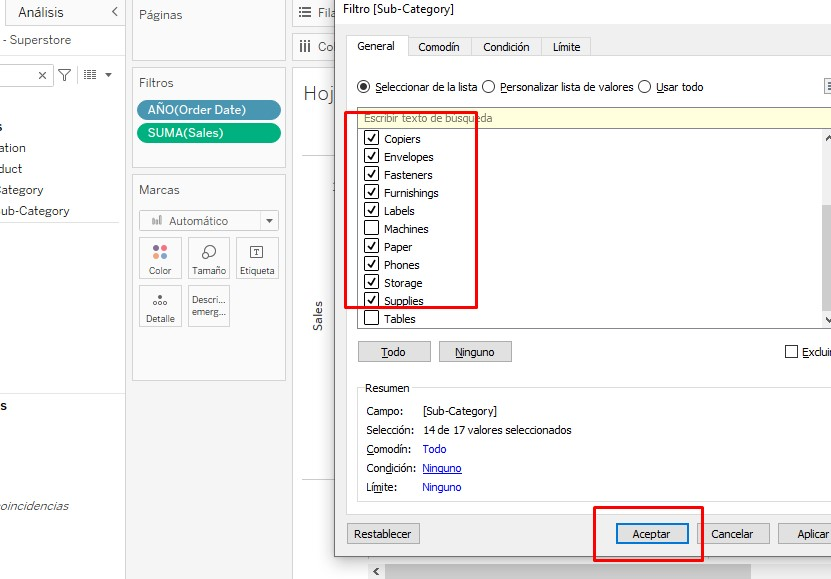
\includegraphics[width=10cm]{./IMAGENES/4.3.1}
\section
%%-----------------------------------------------------------------------------
 	
\section{Vista de mapa}

	\subsection{Crear una vista de mapa}
	\begin{itemize}
		\item Las vistas de mapa son beneficiosas cuando buscamos datos geográficos (el campo
		Región). En el ejemplo actual, Tableau reconoce automáticamente que los campos
		País, Estado, Ciudad y Código postal contienen información geográfica
		
		1. Crea una nueva hoja de trabajo.
		2. Agregue State y Country en el panel Datos a Detail en la tarjeta Marcas. Obtenemos la
		vista del mapa.\\
		\\	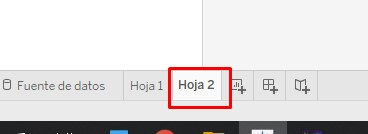
\includegraphics[width=10cm]{./IMAGENES/5.1}
		3. Arrastre Region a la Filters estantería y luego filtre hacia abajo Southsolo. La vista del
		mapa ahora se acerca solo a la región Sur y una marca representa cada estado.
		4. Arrastre la Sales medida a la Colorpestaña de la tarjeta Marcas. Obtenemos un mapa relleno\\
		con los colores que muestra el rango de ventas en cada estado.\\
		5. Podemos cambiar el esquema de color haciendo clic Color en la tarjeta Marcas y
		seleccionando Edit Colors. Podemos experimentar con las paletas disponibles.\\
		6. Observamos que Florida se está desempeñando mejor en ventas. Si pasamos el cursor sobre\
		Florida, muestra un total de 89,474 USD en ventas, en comparación con Carolina del Sur, por
		ejemplo, que tiene solo 8,482 USD en ventas. Evaluemos el rendimiento a Profit estas
		alturas, ya que las ganancias son un mejor indicador que las ventas por sí solas.\\
		7. Arrastre Profit hacia Color en la tarjeta Marcas. Ahora vemos que Tennessee, Carolina del
		Norte y Florida tienen ganancias negativas, aunque parecía que les estaba yendo bien en
		Ventas. Cambiar el nombre de la hoja como Profit Map
		
		\\	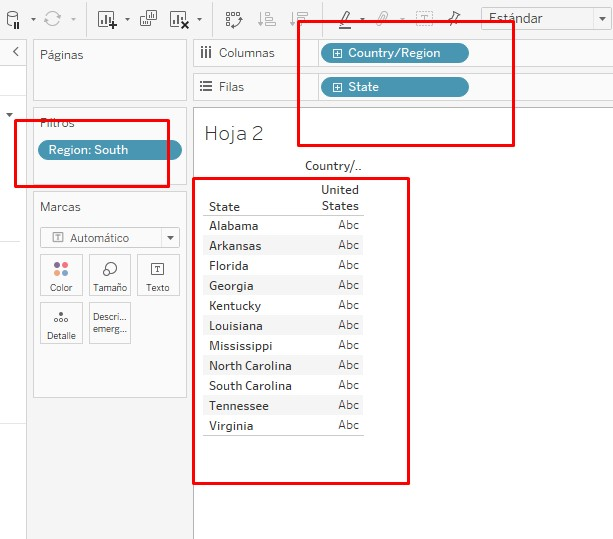
\includegraphics[width=10cm]{./IMAGENES/5.2}
	\end{itemize}
		
	\subsection{Entrar en los detalles}
		\begin{itemize}
			\item 
			1. Duplique la hoja de trabajo Mapa de beneficios y asígnele el nombre Gráfico de barras de
			beneficios negativos.
			\\	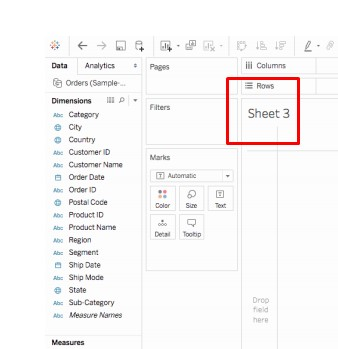
\includegraphics[width=10cm]{./IMAGENES/6.1}
			\\ 2. Haga clic Show Meen la hoja de trabajo Gráfico de barras de ganancias negativas . Show
			Mepresenta el número de formas en que se puede trazar un gráfico entre los elementos 
			mencionados en la hoja de trabajo. De Show Meseleccionar la opción de la barra horizontal y
			los cambios a vista horizontal de las barras verticales de forma instantánea.
			\\ 3. Podemos seleccionar más de una barra a la vez simplemente haciendo clic y arrastrando el
			cursor sobre ellas. Queremos centrarnos únicamente en los tres estados, es decir, Tennessee,
			Carolina del Norte y Florida. Por lo tanto, solo seleccionaremos las barras correspondientes.
			Learn More
			Creación de jerarquías Las
			jerarquías son útiles cuando queremos agrupar campos similares para poder profundizar
			rápidamente entre los niveles de la visualización.
			\\	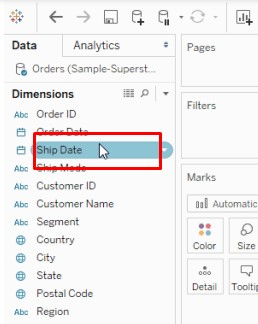
\includegraphics[width=10cm]{./IMAGENES/6.2}
			\\ 1. En el panel Datos, arrastre un campo y suéltelo directamente encima de otro campo o haga clic
			con el botón derecho en el campo y seleccione
			\\ 2. Arrastre cualquier campo adicional a la jerarquía. Los campos también se pueden reordenar en
			la jerarquía simplemente arrastrándolos a una nueva posición. En la visualización
			actual. Crearemos las siguientes jerarquías: Ubicación, Pedido y Producto.
			\\ 4. En el estante de filas, haga clic en el icono con forma de más en el Statecampo para desglosar
			el Citynivel.
			\\	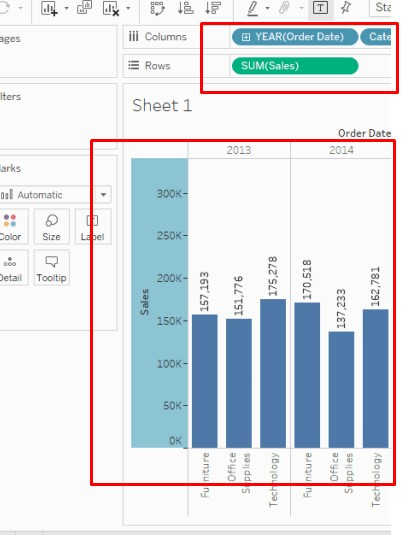
\includegraphics[width=10cm]{./IMAGENES/6.3}
			\\ 1. Eso es una gran cantidad de datos. Podemos usar N-Filter para filtrar y revelar los que tienen
			un desempeño más débil. Para eso, arrastre Citydesde el Datapanel al estante Filtros. Haga
			clic en el campo Por y luego haga clic en el Top menú desplegable y seleccione Bottom para
			revelar los resultados más bajos . Escriba 5 en el cuadro de texto para mostrar los 5 mejores
			resultados en el conjunto de datos.
			\\	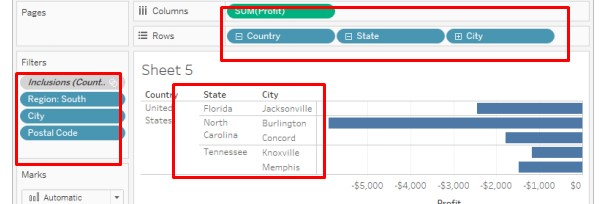
\includegraphics[width=10cm]{./IMAGENES/6.4}
		
    	\end{itemize}
    
    
    
    
    
\section

\section{Tablero}
	\subsection{Crear un tablero}
	\begin{itemize}
		\item 
		1. Haga clic en el New dashboard botón.
		\\ 2. Arrastra Sales in the South al tablero vacío
			\\	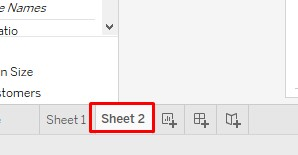
\includegraphics[width=10cm]{./IMAGENES/7.1.1}
		\\ 3. Arrastre Profit Map al tablero y suéltelo encima de Ventas en la vista Sur. Ambas vistas se
		pueden ver a la vez. Para poder presentar los datos de manera que otros puedan entenderlos,
		podemos organizar el tablero a nuestro gusto.
			\\	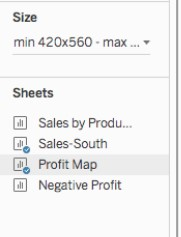
\includegraphics[width=5cm]{./IMAGENES/7.1.2}
		\\ 4. En la Sales Southhoja de trabajo en la vista del tablero, haga clic debajo de Regiony
		borre Show Header. Repita el mismo proceso para todos los demás encabezados. Esto ayuda a
		enfatizar solo lo que se necesita y oculta la información no tan importante.
			\\	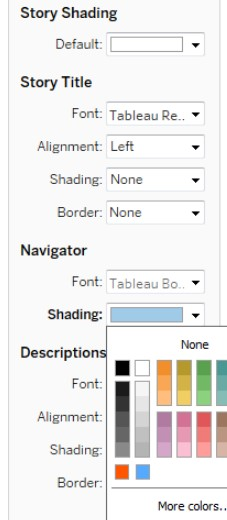
\includegraphics[width=5cm]{./IMAGENES/7.1.2.5}
		\\ 5. En el Profit Map, Ocultar el título también y realizar los mismos pasos para el Sales
		Southmapa.
			\\	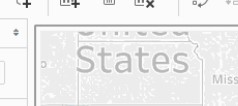
\includegraphics[width=10cm]{./IMAGENES/7.1.3}
		\\ 6. Podemos ver que la Sub-Categorytarjeta de filtro y Year of Order Datese han repetido
		en el lado derecho. Eliminemos los extras simplemente tachándolos. Finalmente, haga clic en
		el Year of Order Date. Aparece una flecha desplegable y seleccione la opción de Single 
		Value (Slider). Ahora deja que la magia se desarrolle. Experimente eligiendo diferentes
		años en el control deslizante y las Ventas también variarán en consecuencia.
		 	\\	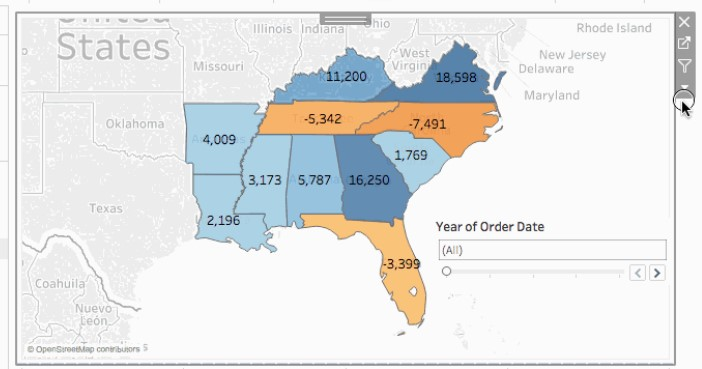
\includegraphics[width=10cm]{./IMAGENES/7.1.4}
		\\ 7. Arrastre el SUM(Profit) filtro a la parte inferior del panel debajo de Ventas en el sur para
		obtener una mejor vista.
		
		 	\\	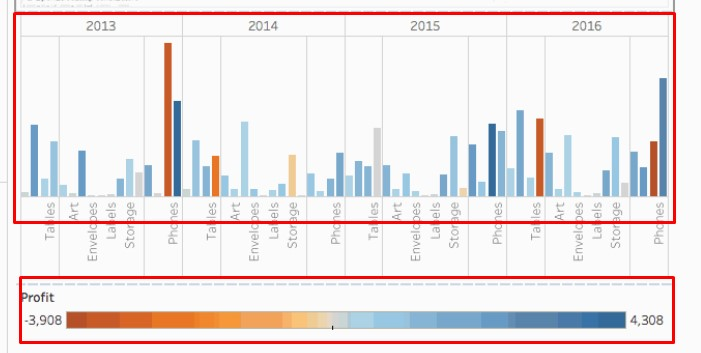
\includegraphics[width=10cm]{./IMAGENES/7.1.5}
	\end{itemize}

		\subsection{Añadien		do interactividad}
			\begin{itemize}
				\item 
					1. Comencemos con el Profit Map. Al hacer clic en el mapa, Use as
					filter aparece un icono en la parte superior derecha. Haz click en eso. Si seleccionamos
					cualquier mapa, las Ventas correspondientes a ese estado se resaltarán en el SalesSouthmapa.
					\\ 2. Para el Year of Order Date, haga clic en la opción desplegable y vaya a Apply to
					Worksheets > Selected Worksheets. Se abre un cuadro de diálogo. Seleccione
					la Allopción seguida de OK. ¿Qué hace esta opción? Aplica filtros a todas las hojas de trabajo
					que tienen la misma fuente de datos.
					\\ 3. Explore y experimente. En la visualización a continuación, podemos filtrar el Sales
					Southmapa para ver los productos que se venden solo en Carolina del Norte. Luego, podemos
					explorar fácilmente las ganancias anuales.
					\\ 4. Cambie el nombre del panel a Regional Sales and Profit.
			\end{itemize}
\section

\section{Historia}
	\subsection{Construyendo una historia}
			\begin{itemize}
				\item 
				1. Haga clic en el New story botón.
				\\ 2. Desde el panel Historia a la izquierda, arrastre la Sales in the South hoja de trabajo
				(creada anteriormente) a la vista.
					\\	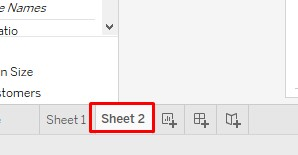
\includegraphics[width=10cm]{./IMAGENES/7.1.1}
				\\ 3. Edite el texto en el cuadro gris sobre la hoja de trabajo. Este es el título. Nómbrelo como Sales
				and profit by year.
					\\	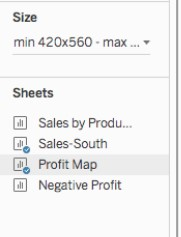
\includegraphics[width=7cm]{./IMAGENES/7.1.2}
				\\ 4. Las historias son bastante específicas. Aquí contaremos una historia sobre la venta de máquinas
				en Carolina del Norte. En el panel Historia, haga clic en Duplicate para duplicar el primer
				título, o incluso puede crear uno nuevo.
					\\	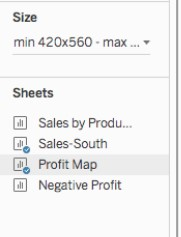
\includegraphics[width=10cm]{./IMAGENES/7.1.2.1}
				\\ 5. En el Sub-Category, select solo filtro Machines. Esto ayuda a medir las ventas y los
				beneficios de las máquinas por año.
				
					\\	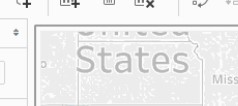
\includegraphics[width=10cm]{./IMAGENES/7.1.3}
				\\ 6. Cambie el nombre del título a Machine sales and profit by year.
					\\	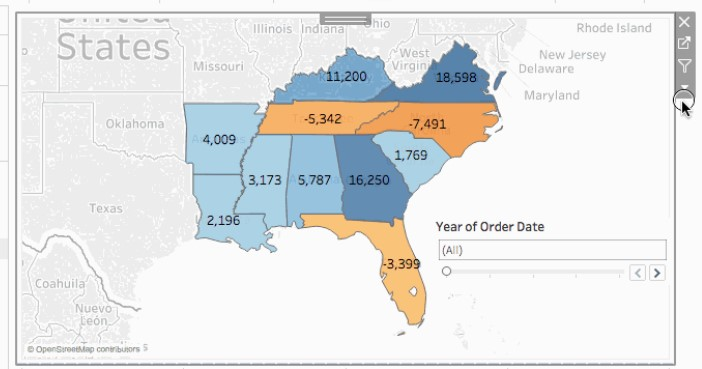
\includegraphics[width=10cm]{./IMAGENES/7.1.4}
			\end{itemize}
		
		\subsection{Conclusiones}
			\begin{itemize}
				\item 1. En el panel Historia, seleccione Blank. Arrastre el panel ya creado Regional Sales and
				Profit al lienzo.
				 		\\	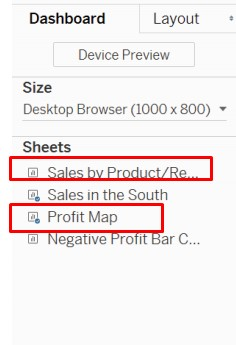
\includegraphics[width=5cm]{./IMAGENES/7.2.1}
				\\ 2. Subtitúlelo como Low performing items in the South.
				\\ 3. Seleccione Duplicate para crear otro punto de la historia con el panel de ganancias
				regionales. Seleccione Carolina del Norte en el gráfico de barras, ya que estamos interesados en
				mostrar más al respecto.
					\\	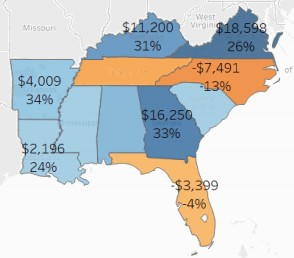
\includegraphics[width=5cm]{./IMAGENES/7.2.2}
				\\ 4. Seleccione Todos los años.
				\\ 5. Agregar un título para mayor claridad, como, Profit in NC : 2013-2016.
				\\ 6. Seleccione cualquier año como 2014. Agregue un título, por ejemplo, Profit in NC :
				2014y luego haga clic en la pestaña Duplicar. Repita el mismo paso para todos los años
				restantes.
				\\ 7. Haz clic en el modo de presentación y deja que se story desarrolle.
					\\	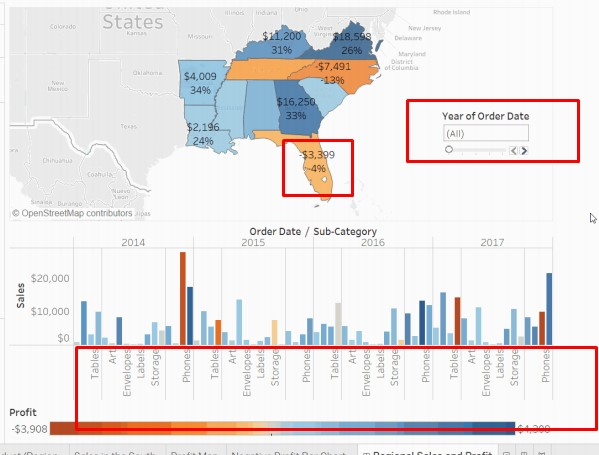
\includegraphics[width=10cm]{./IMAGENES/7.2.3}
			\end{itemize}
\section

\section{Integración de Tableau con R, Python y SQL}
		
		\subsection{Tableau y R}
			\begin{itemize}
				\item 
				Abra el libro de trabajo de Tableau y conéctese a los datos de la supertienda de muestra.
				
						\\	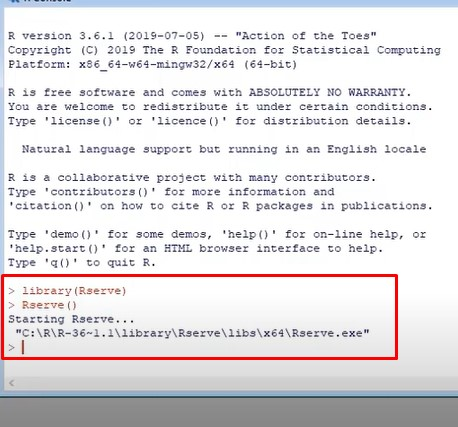
\includegraphics[width=10cm]{./IMAGENES/8.1}
				\\ 2. Conéctese a Rserve. Una vez que Tableau Desktop está conectado a Rserve, puede invocar el
				motor R a través de campos calculados.
				\\	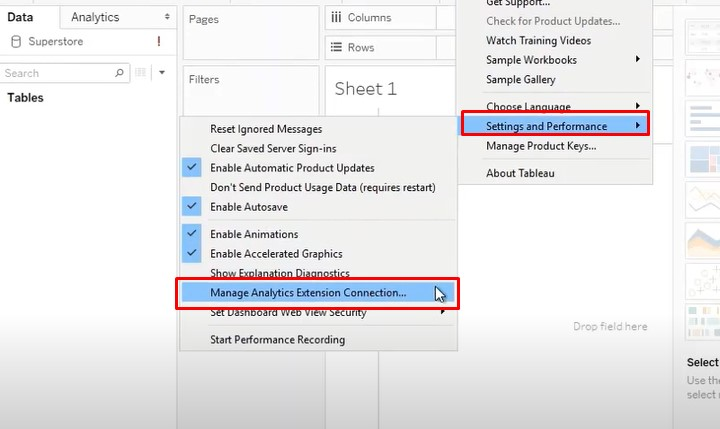
\includegraphics[width=10cm]{./IMAGENES/8.2}
				\\ 3. Ahora crearemos un campo calculado llamado Beneficio esperado.
				Hay cuatro funciones disponibles para usar con R y todas comienzan con la palabra script. Las
				funciones son:
				\\	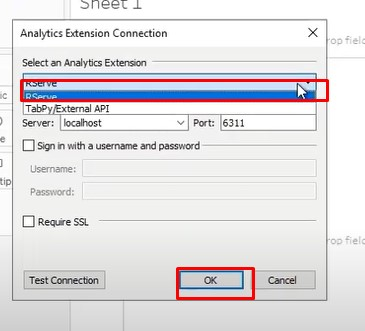
\includegraphics[width=10cm]{./IMAGENES/8.3}
				\\	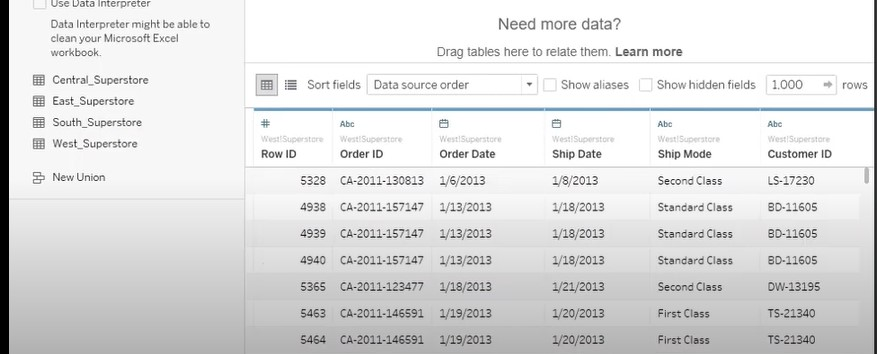
\includegraphics[width=10cm]{./IMAGENES/8.4}
				
				\\ 4. Abra el campo calculado e inserte el siguiente script.
				\\ 5. SCRIPT_REAL("fit <- lm(.arg1 ~ .arg2 + .arg3 + .arg4)
				\\	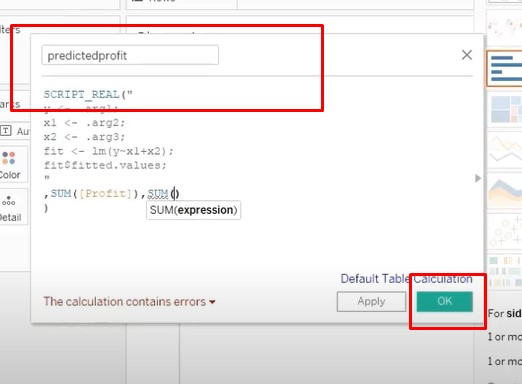
\includegraphics[width=10cm]{./IMAGENES/8.5}
				\\ 6. fit$fit
				
				\\ 8. 8. SUM([Profit]), AVG([Sales]), AVG([Quantity]), AVG([Discount]))
					\\	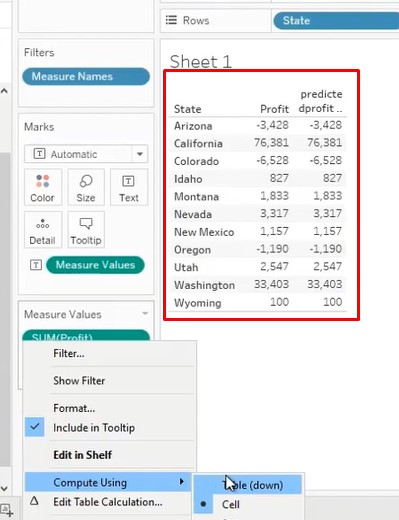
\includegraphics[width=10cm]{./IMAGENES/8.6}
			\end{itemize}	
		
		\subsection{Tableau y Python}
			\begin{itemize}
				
				\item Conectando Tableau con TabPy
				
					\\	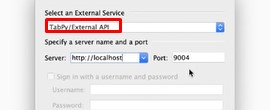
\includegraphics[width=10cm]{./IMAGENES/9.1}
				\item Analisis de sentimiento con taby
					\\	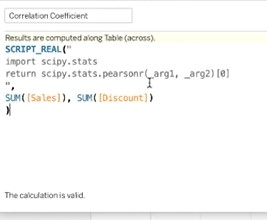
\includegraphics[width=10cm]{./IMAGENES/9.1.2}
					
				
					\\	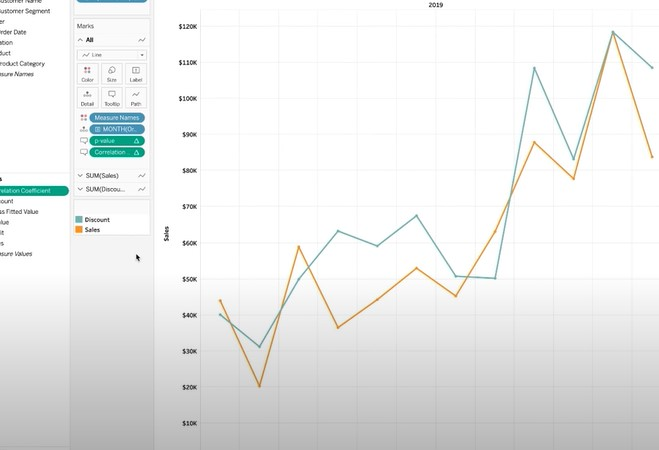
\includegraphics[width=10cm]{./IMAGENES/9.2}
			\end{itemize}
	
		\subsection{Tableau y SQL Server}
			\begin{itemize}
				\item 
				1. Inicie sesión en SQL Server
					\\	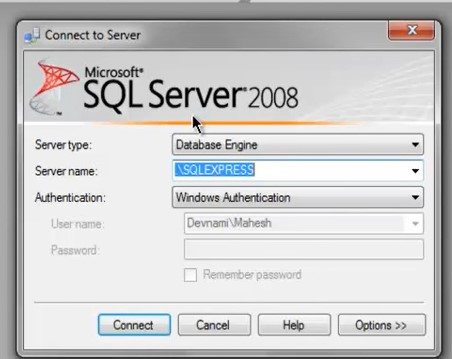
\includegraphics[width=10cm]{./IMAGENES/10.1}
				\\ 2. Abra Tableau Desktop y, en Servidores, conéctese a MS SQL.
					\\	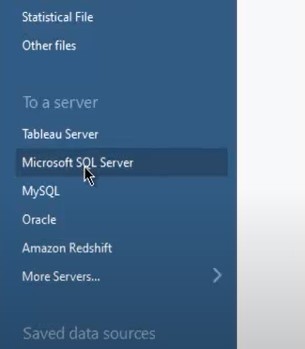
\includegraphics[width=10cm]{./IMAGENES/10.2}
				\\ 3. Pegue el nombre del servidor en el cuadro de diálogo que se abre y haga clic en Aceptar. Esto
				conecta Tableau con SQL Server. Seleccione la base de datos de su elección. En este ejemplo,
				elegimos salesDB. También podemos seleccionar de una lista de TABLAS, por ejemplo,
				Registro de ventas. La tabla se importa al entorno de Tableau. Ahora podemos optar por extraer 
				todos los datos o una parte de ellos a una nueva hoja de trabajo. Incluso podemos especificar el
				número de filas a extraer.
					\\	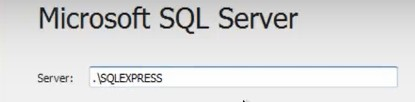
\includegraphics[width=10cm]{./IMAGENES/10.3}
						\\	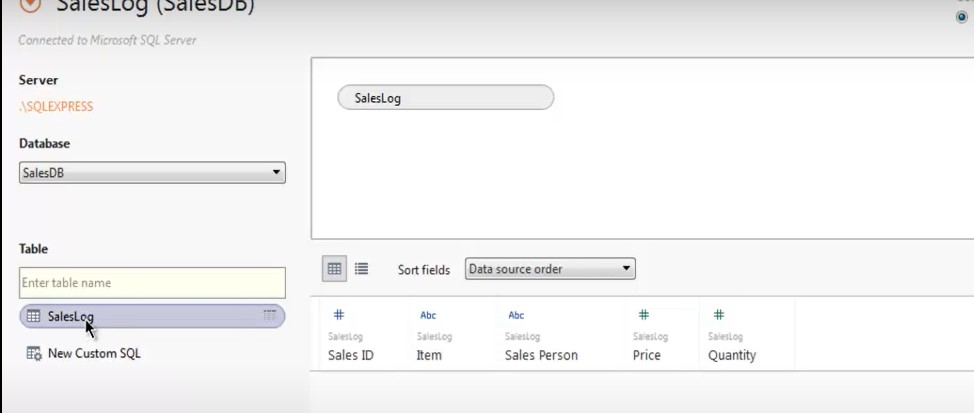
\includegraphics[width=10cm]{./IMAGENES/10.4}
				\\ 4. En la nueva hoja de trabajo tenemos los datos extraídos de MS SQL, desde aquí podemos
				trabajar con ella como cualquier otra hoja de trabajo de Tableau.
					\\	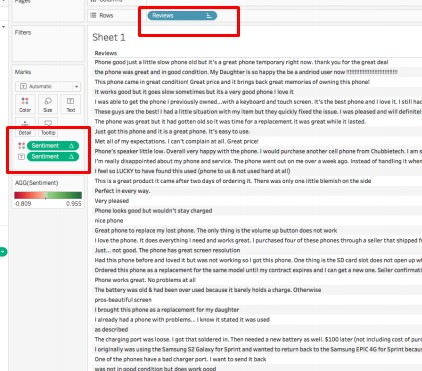
\includegraphics[width=10cm]{./IMAGENES/10.5}
			\end{itemize}
\section

\section{Conclusiones}
		\begin{itemize}
		\item Tableau simplica mucho el trabajo de analizis de negocios, y lo mejor es que se pueden utilizan tecnologias poderosas como python o sqlserver para el analisis mas avanzado de estos.
		\end{itemize}
\section
%%----------------------------------------------------------------------------------------------------------------------------------------------------------
%%FIN Marco Teórico




%CONCLUSIONES







	
	
%\citep{referenciarobles2}  


\end{document}

